\begin{activity} \label{A:4.1.1}  Suppose that a person is walking in such a way that her velocity varies slightly according to the information given in the table below and graph given in Figure~\ref{F:4.1.Act1}.
\begin{center} 
\begin{tabular}{c|c|c|c|c|c|c|c|c|c}
%\hline
$t$ & 0.00 & $0.25$ & $0.50$ & $0.75$ & 1.00 & $1.25$ & $1.50$ & $1.75$ & $2.00$ \\ \hline %\hline
$v(t)$ & $1.500$ & $1.789$ & $1.938$ & $1.992$ & $2.000$ & $2.008$ & $2.063$ & $2.211$ & $2.500$ \\ %\hline
\end{tabular}
\end{center}
\begin{figure}[h]
\begin{center}
\scalebox{0.9}{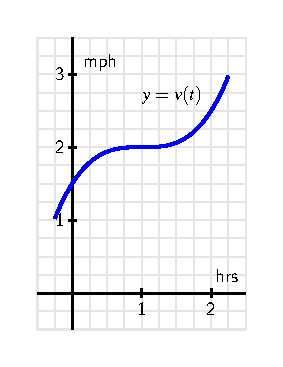
\includegraphics{figures/4_1_Act1.eps}}
\end{center}
\caption{The graph of $y = v(t)$.} \label{F:4.1.Act1}
\end{figure}
\ba
	\item Using the grid, graph, and given data appropriately, estimate the distance traveled by the walker during the two hour interval from $t = 0$ to $t = 2$.  You should use time intervals of width $\triangle t = 0.5$, choosing a way to use the function consistently to determine the height of each rectangle in order to approximate distance traveled.
	\item How could you get a better approximation of the distance traveled on $[0,2]$?  Explain, and then find this new estimate.
	\item Now suppose that you know that $v$ is given by $v(t) = 0.5t^3-1.5t^2+1.5t+1.5$. Remember that $v$ is the derivative of the walker's position function, $s$.  Find a formula for $s$ so that $s' = v$.
	\item Based on your work in (c), what is the value of $s(2) - s(0)$?  What is the meaning of this quantity? 
\ea
\end{activity}
\begin{smallhint}
\ba
	\item For instance, the approximate distance traveled on $[0,0.5]$ can be computed by $v(0) \cdot 0.5 = 1.5 \cdot 0.5 = 0.75$ miles.
	\item Think about the possibility of using a larger number of rectangles.
	\item If $v(t) = t^3$ and we seek a function $s$ such that $s' = v$, note that $s$ has to involve $t^4$.
	\item Observe that this quantity is measuring a change in position.
\ea
\end{smallhint}
\begin{bighint}
\ba
	\item For instance, the approximate distance traveled on $[0,0.5]$ can be computed by $v(0) \cdot 0.5 = 1.5 \cdot 0.5 = 0.75$ mile, while the approximate distance on $[0.5,1]$ can be computed by $v(0.5) \cdot 0.5 = 1.9375 \cdot 0.5 = 0.9688$.
	\item Think about the possibility of using a larger number of rectangles that are narrower in width.
	\item If $v(t) = t^3$ and we seek a function $s$ such that $s' = v$, note that one possible formula for $s$ is $s(t) = \frac{1}{4}t^4$.
	\item Observe that this quantity is measuring a change in position.  How is its value connected to other earlier work you've done?
\ea
\end{bighint}
\begin{activitySolution}
\ba
	\item Using rectangles of width $\triangle t = 0.5$ and choosing to set the heights of the rectangles from the function value at the left end of the interval, we see the following graph and find the sum of the areas of the rectangles to be
	\begin{center}
		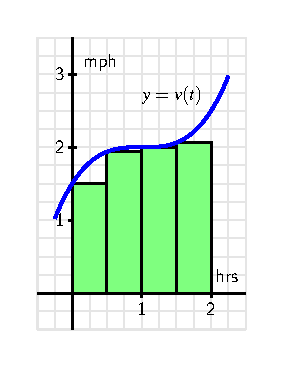
\includegraphics{figures/4_1_Act1Soln.eps}
	\end{center}
	\begin{eqnarray*}
	A & = & v(0.0) \cdot 0.5 + v(0.5) \cdot 0.5 + v(1.0) \cdot 0.5 + v(1.5) \cdot 0.5 \\
	   & = & 1.500 \cdot 0.5 + 1.9375 \cdot 0.5 +  2.000 \cdot 0.5 + 2.0625 \cdot 0.5 \\
	   & = & 3.75
	\end{eqnarray*}
	Thus, the distance traveled is approximately $D \approx 3.75$ miles.
	\item It appears that a better approximation could be found using narrower rectangles.  If we move to 8 rectangles of width $0.25$, similar computations show that $D \approx 3.875$.
	\item By thinking about how the power rule for differentiation works, we can undo this rule and find a position function $s$ whose derivative is $v$.  For instance, since $\frac{d}{dt}[t^4] = 4t^3$, we see that $\frac{d}{dt}[\frac{1}{8}t^4] = \frac{1}{2}t^3$.  Thus, if we let 
	$$s(t) = \frac{1}{8}t^4 - \frac{1}{2} t^3 + \frac{3}{4} t^2 + \frac{3}{2}t,$$
	then it is straightforward to check that $s'(t) = \frac{1}{2}t^3 - \frac{3}{2}t^2 + \frac{3}{2}t + \frac{3}{2}$, which is precisely the formula for $v(t)$ that we were given.
	\item By the rule found in (c) for $s$, we have that $s(2) - s(0) = \frac{1}{8}2^4 - \frac{1}{2}2^3 + \frac{3}{4}2^2 + \frac{3}{2} 2 = 2 - 4 + 3 + 3 = 4$.  This is the change in the walker's position over the time interval $[0,2]$, and since the velocity is always positive, this is actually the exact distance traveled.  We see how both earlier estimates ($3.75$ and $3.785$) are good approximations to this value.
\ea
\end{activitySolution}
\aftera